\documentclass[11pt]{article}
\usepackage{graphicx}    % needed for including graphics e.g. EPS, PS
\usepackage{epstopdf}
\usepackage{amsmath}
\usepackage{hyperref}
\usepackage{xspace}
\usepackage{mathtools}
\usepackage{tikz}
\usepackage{epsfig}
\usepackage{float}
\usepackage{natbib}
\usepackage{subfigure}
\usepackage{setspace}
\usepackage{tabularx,ragged2e,booktabs,caption}

\usepackage{wrapfig}

\setlength{\oddsidemargin}{0.1in}
\setlength{\textwidth}{7.25in}

\setlength{\topmargin}{-1in}     %\topmargin: gap above header
\setlength{\headheight}{0in}     %\headheight: height of header
\setlength{\topskip}{0in}        %\topskip: between header and text
\setlength{\headsep}{0in}        
\setlength{\textheight}{692pt}   %\textheight: height of main text
\setlength{\textwidth}{7.5in}    % \textwidth: width of text
\setlength{\oddsidemargin}{-0.5in}  % \oddsidemargin: odd page left margin
\setlength{\evensidemargin}{0in} %\evensidemargin : even page left margin
\setlength{\parindent}{0.25in}   %\parindent: indentation of paragraphs
\setlength{\parskip}{0pt}        %\parskip: gap between paragraphs
\setlength{\voffset}{0.5in}

\newcommand{\IDK}{*** I DON'T KNOW THIS WORD***}

% Useful commands:

% \hfill		aligns-right everything right of \hfill

\begin{document}
\doublespacing
\title{Radiation Damage in FW and Blanket Structural Materials and Superconducting Magnetic Materials}
\author{M. Abdou \\
Department of Mechanical and Aerospace Engineering \\
University of California Los Angeles, USA\\
}
\maketitle

\section{Page 2}
\subsection{Structural materials}
\begin{itemize}
\item First wall
\item Blanket
\item Other components
\end{itemize}
Candidates: SS, FS, V-alloy, Nb-alloy, M-alloy

Key Problems:
\begin{enumerate}
\item Radiation damage by intense neutrons
\item Radioactivity
\end{enumerate}

For First Wall:
Additional problem:
Surface effects: Intense bombardments by charged particles (H,$\alpha$, impurities) result in surface erosion (sputtering physical \& chemical, blistering, etc.)

For the next two lectures, we will focus on radiation damage and radioactivity issues.

\section{Page 3}
Additional definitions:

Fluence = $\Phi t_{op}$

\begin{equation}
	\text{Fluence} = \Phi t_{op}
\end{equation}

\begin{equation}
	F = \text{plant availability} = \frac{\text{operating time}}{\text{operating time + shutdown time}}
\end{equation}

Integrated neutron wall load

\begin{align}
I_w &= P_{nw} t_{op},  \qquad \qquad [MW y/m^2]     \\
	&= P_{nw} t F
\end{align}

Commonly we measure first wall life in units of $MW y/m^2$
Aspect Ratio for a tokamak = $A$.

\begin{equation}
	A = \frac{\text{(plasma) major radius}}{\text{(plasma) minor radius}}
\end{equation}

\begin{figure}[!htp]
\centering
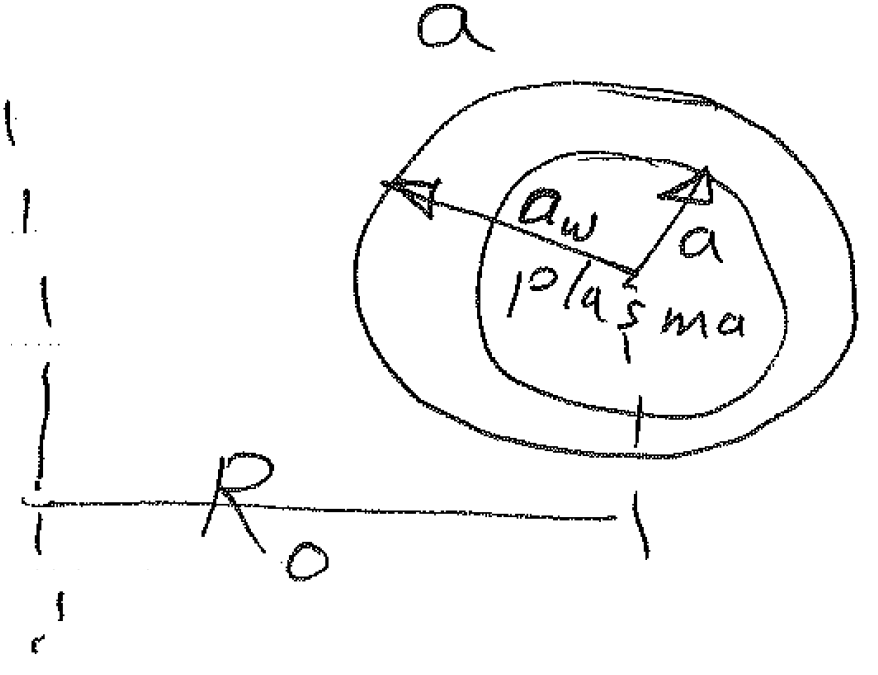
\includegraphics[width=0.45\textwidth]{figs/fig1.png}
\caption[width=\textwidth]{Major and minor radius of toroidal reactor}
\label{fig:reactorRadius}
\end{figure}

\section{Page 4}

\subsection{Radiation Damage}
Units

Flux \& Fluence poor measure
Total flux ~ a factor of 10 higher than 14 MeV neutron current

neutron spectrum provides improvement but it is awkward.

Useful units: dpa

\subsection{Atomic Discplacements}
An energetic particle such as a neutron looses its energy either by electronic excitation or by colliding with the lattice atoms. In a collision with the lattice atom an some energy is transferred into this atom if the quantity of energy transferred is larger than the energy binding the atam in its lattice the stuck atom is displaced by the bombarding particle is called the \textit{primary knock-on atom}, (PKA). Become the PKA possesses substantial kinetic energy, it becomes an energetic particle in it own right

\section{Page 5}
and is capable of creating additional lattice displacements. A displaced atom leaves (i.e. a point defect) its proper place leaving a vacancy behind. The displaced atom will eventually appear in the lattice as an interstitial atom (a point defect). The ensemble of point defects created by a single primary knock-on atom is known as \textit{displacement cascade}.

\subsection{Atomic Displacements Calculating}
\begin{equation}
	\text{dpa} = \text{number of displacements per atom}
\end{equation}
\begin{equation}
	\text{dpa} = \left[ \int \Phi(E) \sigma_d (E) dE \right] t_{\text{radiation time}}
\end{equation}
\begin{equation}
	\sigma_d = \text{displacement cross section}
\end{equation}
\begin{equation}
	\sigma_d(E) = \sum_{\text{all atoms}} \text{probability that a collision occurs x the number of atoms displaced by the PKA}
\end{equation}

\section{Page 6}
\begin{equation}
	\sigma_d(E) = \sum_{\text{all atoms}} \sigma_e (E) \int_{E_d}^{T_{max}} P_i(E,T) \nu(T) dT
\end{equation}
\begin{equation}
	\sigma_i = \text{(nuclear) microscopic cross section for reaction i (elastic, inelastic, (n,2n), (n,$\alpha$), etc.)}
\end{equation}
\begin{equation}
	P_i(E,T) = \text{probability that in reaction i induced by a particle (reaction) of energy E, the PKA has a kinetic energy T}
\end{equation}
\begin{equation}
	E_d = \text{displacement energy or the displacement threshhold}
\end{equation}
\begin{equation}
	\nu(T) = \text{number of displacements produced by a primary knock-on with energy T}
\end{equation}

\subsection{Discussion of \texorpdfstring{$E_d$}{}}
In order for the atom to be displaced it must receive a minimum amount of energy. This is called the displacement energy or the displacement threshold, $E_d$. If the energy transfer $T$ is $<E_d$, the stick atom undergoes large amplitude vibration without leaving the partical well forming its stable lattice portion. The vibration energy is quickly

$E_d$ is in the range of 20 to 60 eV for ()

\section{Page 7}
communicated to the nearest neighbors of the stuck atom and appears as a localized source of heat. On the other hand, if $T>E_d$, the stuck atom is able to pass over the potential barrier and move off into the lattice as a displaced atom.

\begin{wrapfigure}{r}{0.5\textwidth}
  \begin{center}
  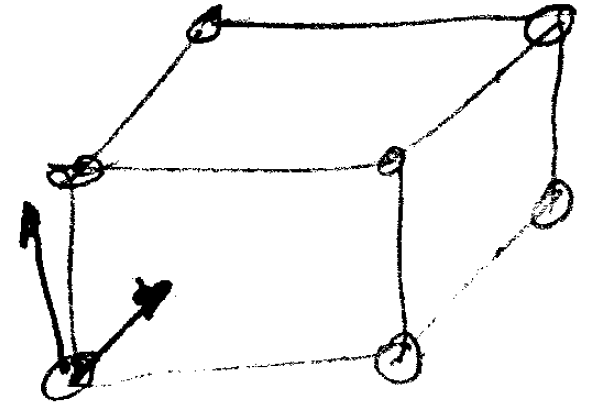
\includegraphics[width=0.45\textwidth]{figs/fig2.png}
  \end{center}
  \caption{Diagram of lattice}
\end{wrapfigure}

In a solid, the potential barrier surrounding a lattice atom in its equilibrioum position \textit{is not uniform} in all directions. Therefore, the energy required to displace an atom depends on the \textit{direction} of the recoil. The direction acquired by the recoil is, of course, dictated by the dynamics of the reactions. In the case of isotropy (isotropic collisions, or high number of bombarding particles that collide isotropically) the direction of the recoil is random or equally probable in all directions.

Therefore, the single value of $E_d$ employed in radiation damage theory is \textit{the spherical average of} $E_d(\theta)$ surrounding the equilibrium lattice site, $E_d$, of course, varies from one material to the other but is generally in the range of 20-60 eV.

\section{Page 8}
$\nu(T)$ is the number of displacements produced by a PKA with energy $T$. The value of $\nu(T)$ should be \textit{independent of the type of collision that produced the PKA}. The crux of the damage producing effect of fast neutrons is the production of displaced atoms by the primary knock-ons. Therefore the calculation of $\nu(T)$ is a very important part of the radiation damage theory.

\begin{wrapfigure}{r}{0.5\textwidth}
  \begin{center}
  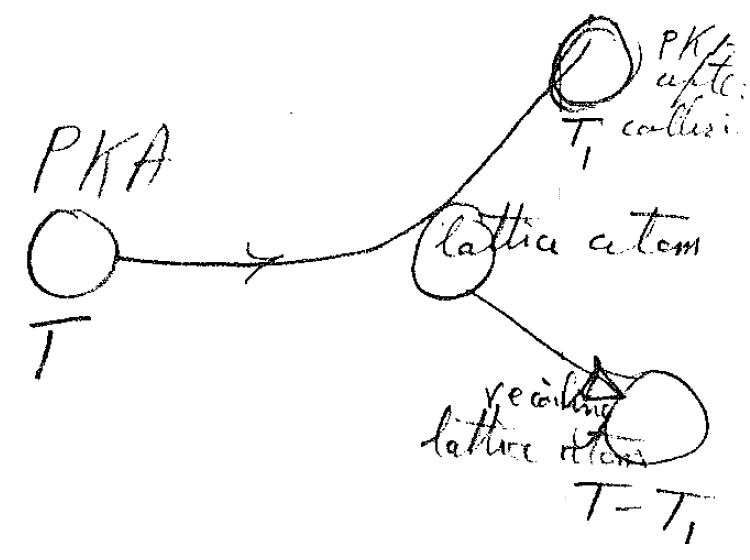
\includegraphics[width=0.35\textwidth]{figs/fig3.png}
  \end{center}
  \caption{PKA collision with lattice}
\end{wrapfigure}

There are several models that have been developed to calculate $\nu(T)$. These models \IDK in the assumptions invoked. However, almost all of them heat the interaction between \IDK a moving atom and the lattice atoms as a sequence of two-body elastic collisions.

There are two important observations you should be aware of regarding this assumption of two-body collisions and elasticity.

\section{Page 9}
\subsection{Handwritten}
The primary collision assumption is quite satisfactory at high interaction energies because the approach distance giving substantial energy transfer are very much smaller than the distances between lattice atoms, \IDK the collisions can be considered to occur between isolated pairs of atoms. However, at low energies appoaching the threshold $E_d$, the cross section for atom-atom interaction is large, and the incoming atom can interact with more than one atom at the same time.

\subsection{Typed}
The collision between a recoil and a lattice atom is often assumed to be elastic, which means that kinetic energy is conserved in the event. Inelasticity can arise from excitation or ionization of the orbital electrons of the atoms involved in the collision. Indeed, interaction of moving atoms or ions with the electrons of the solid constitute the major energy-loss process at high energies. Transfer of energy from the moving atom to electrons does not lead to displacement, only to heat; the low electron mass means that they carry little momentum even though they may be quite energetic. Consequently, it is important to be able to estimage the degree to which the energy of a recoil atom is partitioned between electronic excitation and elastic atom-atom collisions. Only the energy transferred in the latter process is available for causing displacements. Energy is transferred to the electrons in small increments so closely spaced that the process can be regarded as a continuous loss of energy by the moving atom. The atom continues to travel in a straight line but slows down as if it were passing through a viscous medium. The atom-atom interactions, on the other hand, occur at widely spaced intervals; transfer a significant portion of the initial kinetic energy of the moving atom in an essentially instantaneous collision, and produce substantial deflections of the original energetic atom. Consequently, the total energy loss of a moving atom can be accurately separated into two parts: (1) discrete elastic atom-atom encounters which both reduce the energy of the incident atom and produce lattice displacements and (2) a continuous process of electronic excitation which contributes to energy loss but not to displacements.

Not all the energy transferred to a stationary lattice atom by a recoil atom by process 1 is used to displace the former. A substantial portion of the initial energy of the PKA is degraded to heat by atom-atom collisions that do not deliver the requisite displacement energy to the struck atom. In this event the struck atom simply rattles about in its lattice site, ultimately degrading the energy it recieved in the collision to heat.

\section{Page 10}

\section{Typed (on a typewriter)}

The helium or hydrogen production rate in material j due to nuclear transmutation can be calculated from

\begin{equation}
	R_{\alpha}(\vec{\mathbf{r}}) = \int N_j(\vec{\mathbf{r}}) \sigma_{(n,\alpha)j}(E)_{\phi}(\vec{\mathbf{r}},E) dE
\end{equation}
and
\begin{equation}
	R_{H}(\vec{\mathbf{r}}) = \int N_j(\vec{\mathbf{r}}) \sigma_{(n,p)j}(E)_{\phi}(\vec{\mathbf{r}},E) dE
\end{equation}
The helium and hydrogen production rate distributions per 14 MeV neutron leaving the plasma that were calculated for representative blankets are shown in Figures 9.4.2 and 9.4.3.

The helium and hydrogen concentration are commonly expressed in terms of the number of He or H atoms per million lattice atoms, or in atomic parts per million (appm).

Table 9.4.1 summarizes the displacements and He and H concentrations that would result from a neutron fluence of 1 $MW y/m^2$ $(4.48\times 10^{17}$ 14 MeV neutrons per $m^2$) incident upon various materials.
\begin{table}
\centering
\begin{tabular}{|lccc|}
\hline
Material & dpa & appm He & appm H \\
\hline
316SS & 10 & 200  & 540   \\
Nb    & 7  & 24   & 79    \\
Mo    & 8  & 47   & 95    \\
V     & 12 & 57   & 100   \\
C     & 10 & 2700 & small \\
Be    &    & 2800 & 130   \\
\hline
\end{tabular}
\caption{Primary response characteristics (Neutron Fluence of 1 ME $y/m^2$)}
\end{table}


\section{Pages 11-14}

\begin{figure}
  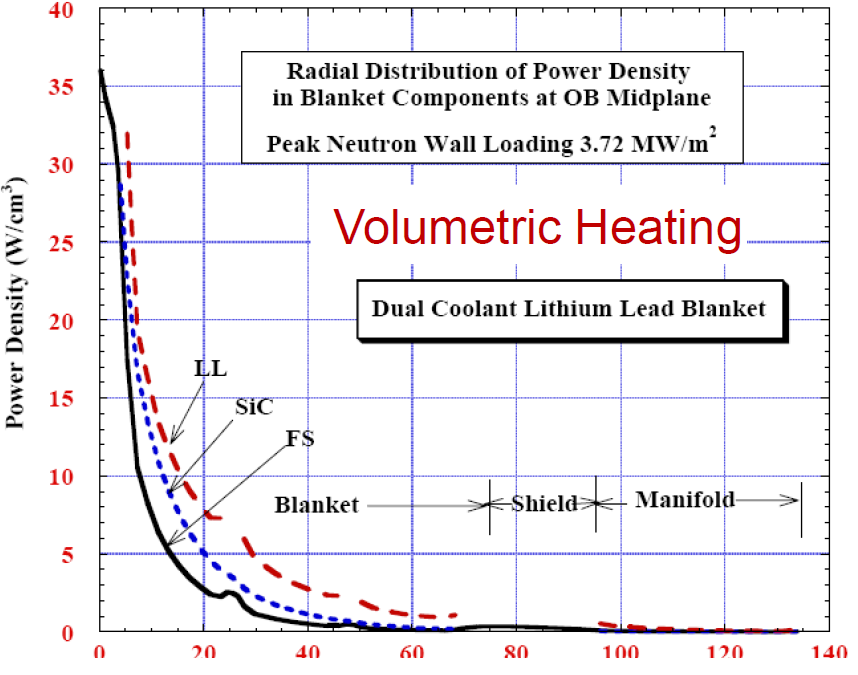
\includegraphics[width=0.45\textwidth]{figs/fig4.png}
  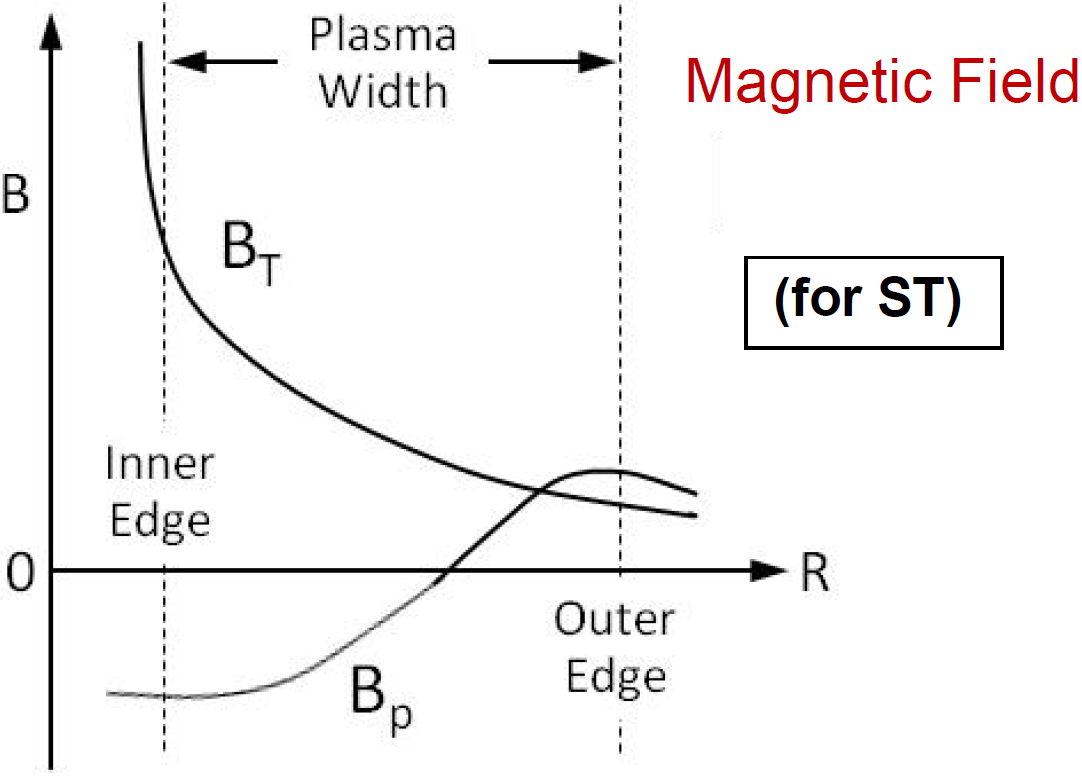
\includegraphics[width=0.45\textwidth]{figs/fig6.png}
  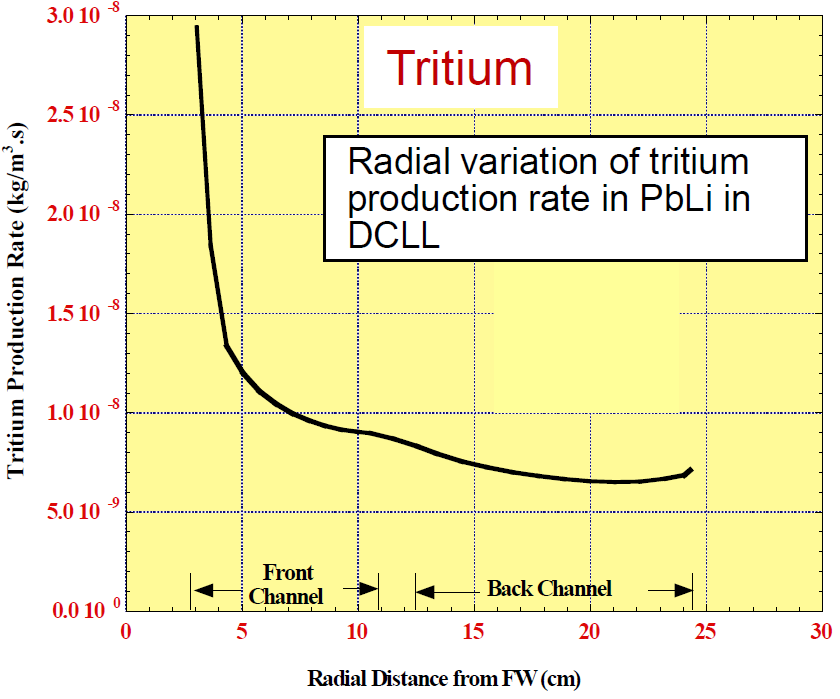
\includegraphics[width=0.45\textwidth]{figs/fig5.png}
  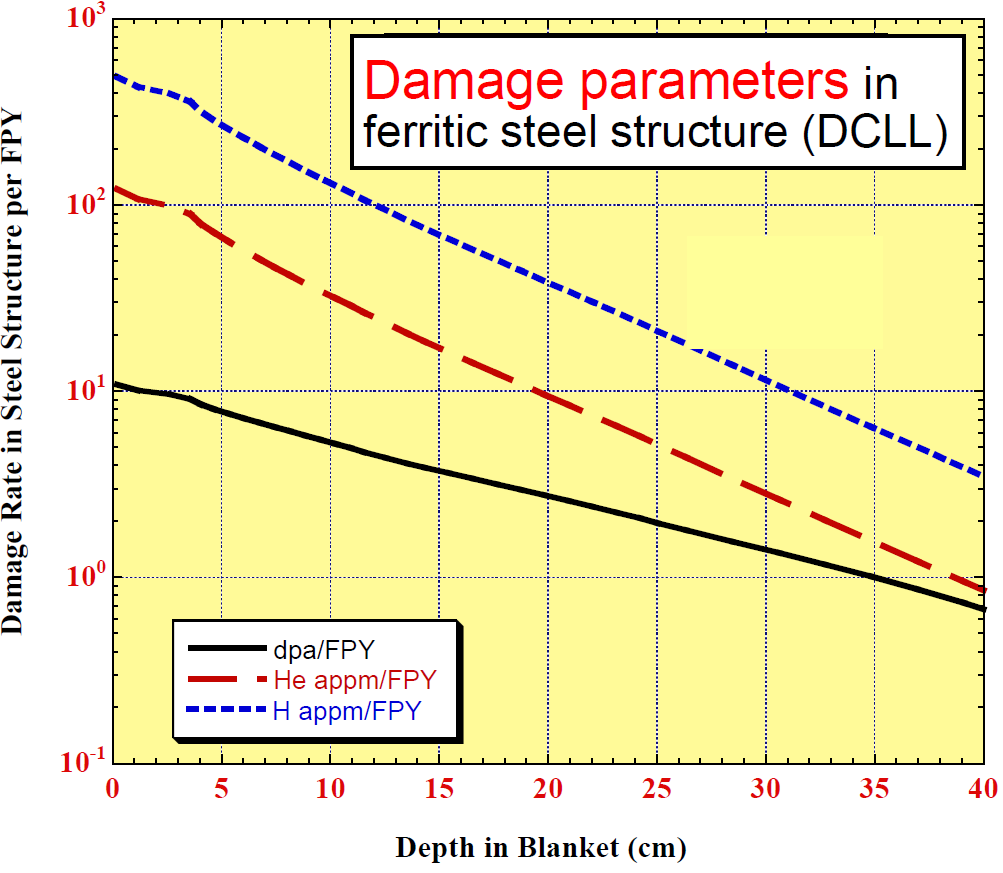
\includegraphics[width=0.45\textwidth]{figs/fig7.png}
  \caption{PKA collision with lattice}
\end{figure}

\begin{figure}
  \centering
  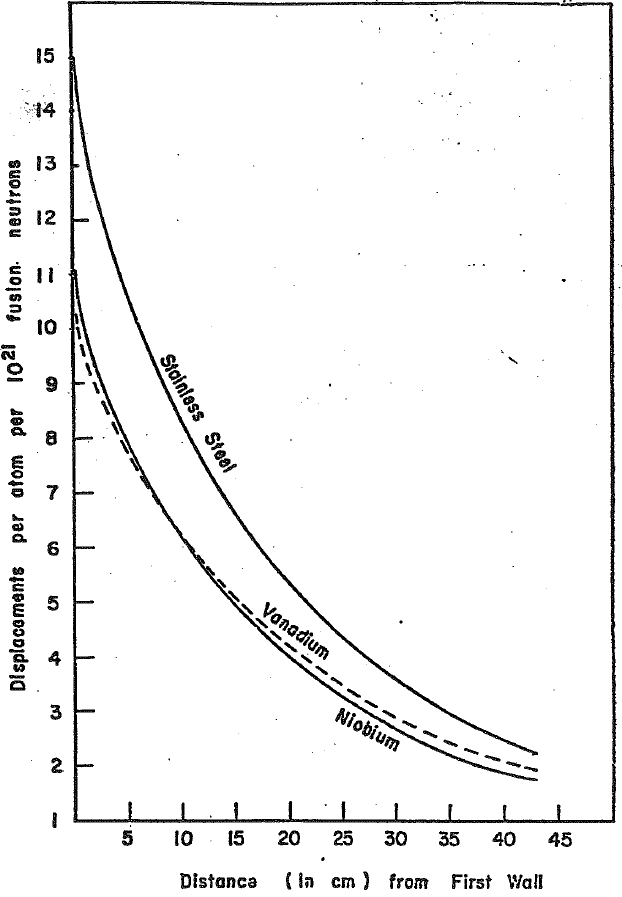
\includegraphics[width=0.45\textwidth]{figs/fig8.png}
  \caption{Comparison of Atomic Discplacement for Vanadium, Niobium and Stainless Steel}
\end{figure}
\begin{figure}
  \centering
  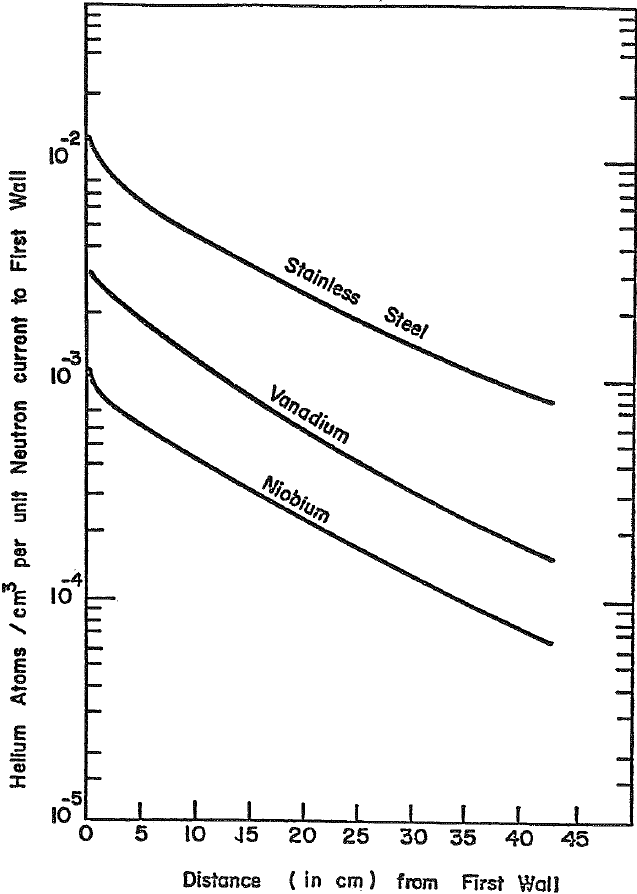
\includegraphics[width=0.45\textwidth]{figs/fig9.png}
  \caption{Comparison of Helium Production in Vanadium, Niobium and Stainless Steel}
\end{figure}
\begin{figure}
  \centering
  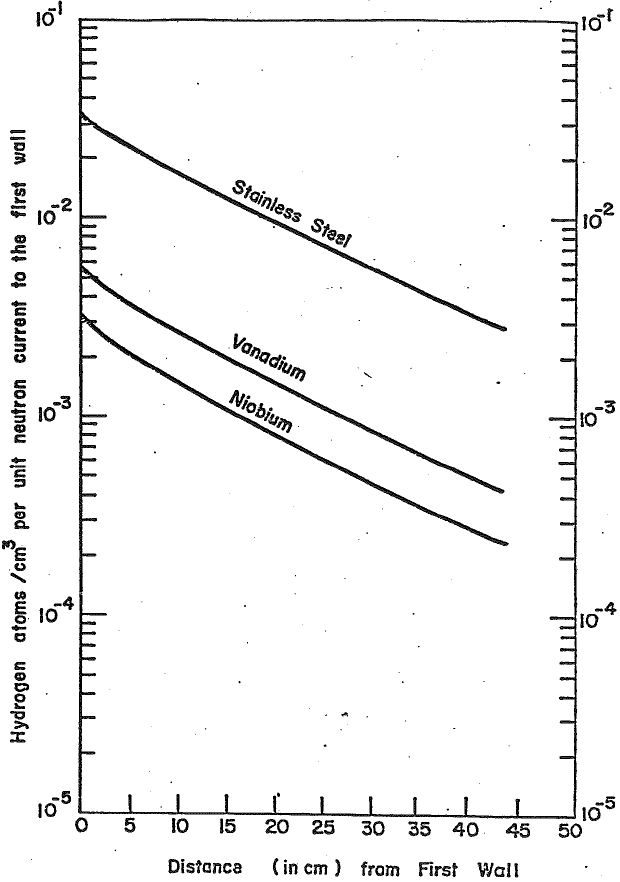
\includegraphics[width=0.45\textwidth]{figs/fig10.png}
  \caption{Comparison of Hydrogen Production in Vanadium, Niobium and Stainless Steel}
\end{figure}

\section{Page 15}
\subsection{Material Properties Changes (radiation effects)}
The primary responses...


\end{document}